\documentclass{article}
\usepackage[utf8]{inputenc}
\usepackage{multicol}
\usepackage{graphicx}
\usepackage{enumitem}
\usepackage{amsmath}
\usepackage{indentfirst}
\usepackage{tabulary}
\usepackage{hyperref}
\usepackage{pdfpages}



\addtolength{\oddsidemargin}{-.875in}
\addtolength{\evensidemargin}{-.875in}
\addtolength{\textwidth}{1.75in}
\addtolength{\topmargin}{-.875in}
\addtolength{\textheight}{1.75in}

\begin{document}
\begin{titlepage}
\begin{center}

    \vspace{3cm}
    {\huge\bfseries Microgravity Electrothermal Liquidation Tunneler (M.E.L.T.) 
    Under Ice Microgravity NExT\par}
    
    \vspace{2cm}
    {\huge The Ice Fishers at UCLA\par}
    {\huge University of California, Los Angeles\par} 
    {\huge 405 Hilgard Avenue\par}
    {\huge Los Angles, CA 90095\par}
    
    \vspace{1cm}
    {\Large Team Contact\par}
    \vspace{.25cm}
    {\large Simon Ng\par}
    {\large ngsimon227@gmail.com\par}
    {\large (414)882-9172\par}
    
    
    \vspace{1cm}
    {\Large Team Members\par}
    \vspace{.25cm}
    {\large\itshape David James - Technical/ Safety\par}
    {\large davidabraham@ucla.edu - 4th Year Computational Mathematics\par}
    \vspace{.25cm}
    {\large\itshape Jenny Wu - Technical/ Safety\par}
    {\large jenny.wu.dalian@outlook.com - 2nd Year Computer Science\par}
    \vspace{.25cm}
    {\large\itshape Simon Ng - Technical/ Safety\par}
    {\large ngsimon227@gmail.com - 1st Year Bioengineering\par}
    \vspace{.25cm}
    {\large\itshape Lou Baya Ould Rouis - Outreach Manager\par}
    {\large loubaya.or@gmail.com - 1st Year Physics\par}
    
    \vspace{1cm}
    {\Large Faculty Advisor \par}
    \vspace{.25cm}
    {\large\itshape Dr. Tsu-chin Tsao \par}
    {\large ttsao@ucla.edu \par}
    {\large (310) 206-2819 \par}
    \vspace{1cm}
    Faculty Signature: \hrulefill


\end{center}
\end{titlepage}

\begin{titlepage}
\tableofcontents
\end{titlepage}

\section{Technical Section}
%Primary Section for the Under Ice Proposal
\subsection{Abstract}
Ice is well known for its ability to entrap microbial life and biomolecules \cite{Knowlton}, and it provides a record of physical history within its stratigraphy. Thus, in the search for life or its components on ice covered ocean worlds such as Europa or Enceladus, it is crucial to be able to take ice core samples with reliability and to preserve the stratigraphy of the samples for later analysis. Our device has two parts, one of which will remain in the rover for stability and another which will extend to the undersurface of the ice sheet. Three electrothermal drills will melt their way into the ice with a heated wire in their tips. They will be pushed by pneumatic pressure. Once the drill is fully extended, the heated wire is pulled through the cross section of the ice, cutting it. Once all of the drills have collected their samples, the extended part of the device will return into the rover. The samples could either be analyzed on board of the rover or on a larger, homebase rover.

\subsection{Design Description}
Our device is designed to take a subaqueous ice sample from an ice sheet. The device is made up of two cylinders. One cylinder ($C_1$) has a height of 1.5" and a diameter of 3"; $C_1$ will stay within the rover. The second cylinder ($C_2$) has a height of 4.5" and a diameter of 3". $C_2$ will be extended as a unit outside of the rover into the marine environment until its top side is flush with the ice sheet above. $C_2$ will extend via buoyancy, and will be attached to $C_1$ with fishing line. In $C_2$, there will be 3 drill wells, each holding an electrothermal, hollow drill, each of which will store its sample within its bore, preventing cross contamination. The drills will push into the ice, melting their way in with a heated nichrome wire in its tip, leaving the center of the ice core frozen. The force pushing each drill into the ice will be provided with pneumatic power via an air hose from $C_1$ to $C_2$ and then separately to each drill well. Each drill well will be isolated from the air hose by a small metal hatch and from the water above by a large metal hatch across the entire cross section of the drill. Upon an automated signal from a pressure gauge in the air hose, the hatches for one drill well will rotate horizontally open, allowing pressurized air into the drill well, increasing the pressure, forcing the drill to melt its way into the ice directly above it. When the drill has melted 3" into the ice, a motor in $C_2$ will coil the wire, pulling the heating wire across the cross through the ice. Then the drill will be pulled back into its drill well with a motor and fishing line. Once the drill is in its well, its two hatches, above and below, will rotate horizontally closed, preventing contamination from the water outside the device and the air below. This process will be repeated one by one with each of the drills. Once all 3 samples have been collected, $C_2$ will be pulled back to $C_1$ by the connecting fishing line. With 3 ice samples collected and secured, the rover will be ready to move on to its next mission. Once the rover has completed its other missions, the ice samples will be remotely analyzed for microbial life and other details of the ocean climate of the planet.

\subsubsection{Device Design}

\paragraph{Cylinder 1 ($C_1$)}

$C_1$ is a hollow cylinder made of 3D printed acrylonitrile-butadiene-styrene ESD7 (ABS) with a diameter of 3" and a height of 1.5". ABS is impact-resistant, tough, non-permeable, non-toxic, low density, relatively inexpensive, and it has a high melting point of 220C \cite{Hamod}. ABS ESD7 is particularly suited to the project because it is resistant to electrostatic discharge, providing extra security given the use of electronic components\cite{Stratasys}. $C_1$ remains at the bottom of the modular instrument bay at all times to provide a point of grounding for $C_2$. $C_1$ contains the input valves for the pneumatic and electric systems, as well as the micro-controller. Additionally, $C_1$ contains three motors with spooled 30 lbs fluorocarbon fishing line, selected for its tensile strength, low elasticity, and resistance to water absorption. The line connects $C_1$ to $C_2$. The motors release line to allow $C_2$ to reach the ice surface. They also coil line to bring $C_2$ back into the instrument bay.

\paragraph{Cylinder 2 ($C_2$)}
$C_2$ is a hollow cylinder made of ABS-ESD7 with a diameter of 3" and a height of 4.5". $C_2$ exits the modular instrument bay, connected to $C_1$ by the fluorocarbon line. $C_2$ contains an evacuated chamber, so when the three motors in $C_2$ release the line, $C_2$ will float up until it is flush with the under-surface of the ice. $C_2$ contains another small electric motherboard as well as the three drill wells, arranged in a triangular form.

\paragraph{Pneumatic System}
The pneumatic system uses ether polyurethane tubing due to its water and corrosion resistance as well as its ability to retain its flexural properties in cold conditions as low as -65\cite{Ann}. The input connector is a Grainger Coupler Plug, item 1HLZ9, and its outermost part is flush with the outer surface of $C_1$. The tubing is coiled outside $C_1$ in a small cylindrical depression of diameter 1". The tubing uncoils with $C_2$ as it extends from $C_1$. When $C_2$ is fully extended, the tubing crosses the aqueous gap to deliver pressurized air to $C_2$ at no more than 18 psig. Within $C_2$, the $\frac{1}{4}$" tubing divides via a 3D printed ABS divider into three tubes, each going to one drill well.



\begin{gather*}
    \sum \vec{F} = m \vec{a} \\
    \vec{F}_g = m \vec{g}\\
    P = \frac{F}{s}
\end{gather*}

\begin{align*}
    \sum \vec{F} &= m \vec{a} \\
    F_P + F_g &= m*a \\
    P*s + m*g &= m*a \\
    P &= \frac{m (a+g)}{s}
\end{align*}

\paragraph{Drill Well}
The three drill wells are made of ABS ESD7, printed as part of $C_2$. Each of the drill wells is identical, with an inside diameter of 0.82" and a depth of 3.50". The well has a $\frac{1}{4}$" diameter hole in the bottom which connects to the polyurethane tubing via threading, allowing the pressurized air to enter the drill well, pushing the drill up into the ice.
\subparagraph{Hatch System}
The drill well begins in a sealed state, with hatches both above it and below it. The hatch above seals the drill from the aqueous environment, preventing contamination prior to retrieving the sample. The hatch below seals the drill well from the pneumatic tubing, giving control of the pressure in the drill well. The hatches are connected, so they open together, simultaneously allowing pressurized air into the drill well and allowing the drill to push up into the ice above. Once the drill has returned into its well, the hatches close together, preventing contamination and stopping the pressurized air from entering the well.
\paragraph{Drill}
The three drills are identical. Each drill has two layers with an evacuated gap in between to provide insulation. At the tip of the drill is a heating wire which serves to melt the ice around the desired ice core sample, allowing the drill the push into the ice.


\begin{gather*}
    Q = \frac{V^2}{R}*t \\
    Q = m*c*\delta T \\
    m = \rho * V \\
    V = s*d \\
\end{gather*}

\begin{align*}
    m &= \rho * s*d \\
    \frac{V^2}{R}*t &= (m*c*\Delta T \\
    &= (\rho * s*d) c * \Delta T \\
    d &= \frac{V^2 * t}{\rho *s*c*\Delta T*R} \\
    \frac{d}{dt}(d) &= \frac{d}{dt}(t)* \frac{V^2}{\rho *s*c*\Delta T*R} \\
    v &= \frac{V^2}{\rho *s*c*\Delta T*R}
\end{align*}

\subparagraph{Heated Drill Tip}
The heating element is $\frac{1}{16}$" diameter nichrome 80/20 wire. The nichrome wire circles completely around the drill tip in a divot, and at its ends, the nichrome wire is connected to a copper wire of the same diameter. The copper wires travel down the melt channel to $C_2$, where the copper wires are attached to a spooling motor. When the drill has extended 3" into the ice, the motor begins coiling the copper wires, pulling the hot nichrome wire out of its divot, into the ice, cutting the ice sample cross wise from its mother ice sheet.
\subparagraph{Drill Body}
Each drill measures 0.817" in diameter and 3.5" in height with two walls. The 0.018" thick outer wall is stainless steel, and the 0.0689" inner wall is ABS ESD7. Stainless steel is the ideal outer wall material due to its resistance to corrosion in a chlorine aqueous environment and its strength under pressure and heat. It also has a thermal conductivity of 50.2W/(mK), so it will be partially heated by the nichrome wire, ensuring that the drill does not freeze in the ice and that pushing into the ice sheet is smooth. ABS ESD7 is the ideal inner wall material due to its high thermal insulation and, inversely, lower thermal conductivity, which is 0.1W/(mK). The space between the two walls is evacuated to further insulate the ice sample. ABS ESD7 also does not attract atomized liquids, helping to preserve the ice sample’s stratigraphy. The body is also attached via fluorocarbon fishing line to a motor in $C_2$, allowing the drill to be retracted into its drill well once its sample is collected. There is also a channel running the length of the drill which allows the melted, displaced water to run out into the aqueous environment. Each drill has two integrated hinges and a clasp to allow the drill to open lengthwise to remove the sample, preserving stratigraphy.

\subsubsection{Requirement Compliance Matrix}
\begin{center}
    \begin{tabulary}{\linewidth}{|L|L|}
    \hline
    Objectives & Method \\
    \hline
    The device shall collect cylindrical samples 0.5" diameter and 3" deep. &
    The inner sheath of each drill that stores the ice is be 0.5" in diameter and 3" deep. \\
    \hline
    The device shall collect, seal, and store at least 1 sample. &
    The device stores each sample in its own sheath within each drill. A hatch seals each drill whenever it is not in the ice sheet. \\
    \hline
    The device shall obtain a subsurface sample from solid and slushy ice. &
    The device melts a path through the ice, solid or slushy, with a heated nichrome 80/20 wire. Once the drill has obtained a 3" sample, the nichrome wire is pulled across the cross section of the sample, separating it from the ice sheet. \\
    \hline
    The device shall minimize cross contamination between samples. &
    Each sample is in its own isolated drill, preventing contamination between samples. \\
    \hline
    The device shall minimize cross contamination by air or water once obtained. &
    The drill containing each sample is covered by a hatch both above and below as soon as it is fully within its drill well, keeping both water and air from contaminating the sample. \\
    \hline
    The device can be operated electrically by no more than 12V. Power to be supplied by the NBL only. &
    The device runs on a micro-controller, and power consumption for the heated wire and the motors is below 10V. \\
    \hline
    The device can have multiple parts that can attach and detach &
    The device consists of two cylinders. One remains in the rover, and the other extends up to the ice sheet to retrieve 3 samples. \\
    \hline
    The device (all parts, in stowed configuration) shall fit within a 3" diameter x 6" long cylinder. &
    The 2 cylinders and 3 drills, when in stowed configuration, makes a cylinder with a 3" diameter and a 6" height. \\
    \hline
    The device (all parts) shall have a dry weight less than 5 lbs. &
    The device's weight will be 4.5 lbs due to the use of light ABS plastic. \\
    \hline
    The device (all parts) shall operate underwater with provided electrical power &
    The device's shell will be made from 3D printed ABS, a non-permeable plastic, and all seams will be sealed with marine adhesive. The device will be compatible with female banana plug connections. \\
    \hline
    The device shall be commanded via general purpose input/output lines (3.3V or 5V compatible), or via a Universal Asynchronous Receiver/ Transmitter (UART-3.3V/5V). & 
    The device runs on a simple DC circuit. \\
    \hline
    The device shall be compatible with a chlorine water environment and a salt-water environment. & 
    The outside of the device is made from ABS and stainless steel, both resistant to chlorine and salt water environments.\\
    \hline
    The device shall operate within an environment from -5$^\circ$C to 30$^\circ$C. &
    All components are safely operable within a range between -40$^\circ$C to 70$^\circ$C, and the outer cylinders are made from ABS, which has a high thermal insulation (0.1W/(mK). \\
    \hline
    \end{tabulary}
\end{center}
\subsubsection{Additional Desires Compliance Matrix}
\begin{center}
    \begin{tabulary}{\linewidth}{|L|L|}
    \hline
    Objectives & Method \\
    \hline
    The device shall be able to collect, seal, and store at least 3 samples. &
    The device has 3 thermal drills, and each drill stores its own ice sample. \\
    \hline
    The device shall maintain the stratigraphy of the sample during collection, containment, and transportation. The sample shall not melt. &
    The drill melts the ice around the sample, leaving the desired sample as solid ice. The drill has 2 walls, with stainless steel on the outside and ABS on the inside for thermal insulation. Additionally, the gap between the walls is evacuated, providing further insulation and maintaining the sample's solid stratigraphy through containment and transportation. \\
    \hline
    The device shall allow for removal of samples for verification that the stratigraphy is maintained &
    The drill opens from the side to allow removal of the sample without risk of compromising stratigraphy. \\
    \hline
    \end{tabulary}
\end{center}
\subsubsection{Manufacturing Plan}

All team members will take the general laboratory safety course to use the student machine shop. All manufacturing will take place at UCLA, so we do not expect any outside machine shop costs.

\begin{center}
    \begin{tabulary}{\linewidth}{|L|L|L|L|}
    \hline
    Material & \ Price \\
    \hline
    Nichrome heating wire ($\frac{1}{16}$") & \$ 22.25 \\
    \hline
    Stainless Steel (0.018" thick)          & \$ 19.36 \\
    \hline
    Steel Industrial Quick Coupler Plug (0.005 lbs)     & \$ 1.65 \\
    \hline
    ABS ESD7 Filament & \$90 \\
    \hline
    30 Lb Fluorocarbon Fishing line & \$13 \\
    \hline
    Ether Polyurethane (5ft.) & \$2.60 \\
    \hline
    Master Bond Supreme 3HT-80 (adhesive for steel-abs) & Not Available \\
    \hline
    3M™ Marine Adhesive Sealant 5200 Fast Cure & \$9.99 \\
    \hline
    Copper Wire & \$8.72 \\
    \hline
    RTV 108 Silicone Rubber Adhesive Sealant & \$9.33 \\
    \hline
    12 Servo motors & \$42 \\
    \hline
    Miscellaneous Electronics & \$40 \\
    \hline
    \end{tabulary}
\end{center}


\subsection{Operations Plan}

The test will begin with the device being submerged and placed on the buoyant platform beneath the ice sheet. Once everything is set, three motors in $C_1$ will unspool fishing line connecting to $C_2$, and $C_2$ will float away from $C_1$ to the undersurface of the ice. 

Once $C_2$ is at the ice, the air pressure will be turned on between 15 and 18 psig. With increasing pressure, pressure gauges within the device will open one drill well hatch system, and the drill will be pushed out of the well by the pressure. At the same time, electricity will be fed to the nichrome heating wire in the tip of the drill, melting the ice as the drill is pushed into it. Once the drill has fully extended, retrieving a 3" sample, the heated wire will be pulled by a spooling motor within $C_2$, pulling the heated wire through the ice cross section. Then, a motor will spool fishing line attached to the bottom of the drill, pulling it back into the drill well. Once the drill is fully in the drill well, the hatches will close, closing out water and pressurized air. The same process will be repeated with the other two drills to obtain a total of 3 samples. At this point the pressurized air can be turned off.

As soon as the three samples are within $C_2$, the three motors in $C_1$ will spool up the fishing line, pulling $C_2$ back to $C_1$. At this point, the electricity can be turned off. The device can be retrieved from the water. Upon land, the drills can be removed from the wells and opened to investigate whether stratigraphy was preserved. The test is then finished.

\subsection{Safety}
%Protect the Rover

This device’s design does not require EVA, and thus potential danger to humans is extremely low. However, safety is still paramount. On a rover mission, it is critical that this device does not cause any compromise to the data being collected by other instruments.

To ensure device safety, both $C_1$ and $C_2$ are made from ABS ESD7, sealed at seams with 3M\textsuperscript{TM} Marine Adhesive Sealant 5200. ABS is impact-resistant, tough, and resistant to electrostatic discharge, ensuring that any stray electric charges within the device will not be transferred to the surrounding water or the rover. Additionally, all internal wiring will be insulated to prevent electric shock in case water does somehow breach either of the cylinders. The copper and nichrome heating wires in the drills are also insulated, preventing electric shock in the water. The female banana plugs will connect with the main circuit board through two walls of ABS ESD7. First, the banana plug wires pass through holes in the outer wall of $C_1$, and then the wires pass through a smaller ABS ESD7 box within $C_1$, providing secondary protection of electrical components. The input wires will be insulated, and the holes they go through will be as small as possible. Once the wires are hooked up through the two walls, any remaining gap between the wire and the wall will be filled with RTV 108 Silicone Rubber Adhesive Sealant, selected for its electrical insulating properties\cite{Ann} \cite{Aquino}. A layer of 3M\textsuperscript{TM} Marine Adhesive Sealant 5200 Fast Cure will be applied over that for its waterproofing quality to ensure that there is no path for water to enter into the electrical circuitry. 

This method will be tested prior to testing in the NBL to verify that it is in fact a barrier to electric shock. In an aquarium, we will make an aqueous solution with 3.5 ppm free chlorine, the maximum level in the NBL. We will submerge our device in the solution and run electricity through the wires to ensure that no water gets in and that there are no unforeseen issues. We will run the procedure at a variety of temperatures from 0$^\circ$C to 30$^\circ$C to ensure safety at all possible water temperatures in the NBL. We will repeat the procedure with a sodium chloride solution to ensure there are no issues with a saltwater environment. If we discover any leaks or other problems, we will redesign our barrier, and then will test it again.

The pneumatic system is in compliance with NBL requirements that all pneumatic elements must be rated for at least 2.5 times our maximum supply pressure, which will be low, no higher than 18 psig. Therefore, our elements must be rated for at least 45 psi, which all elements far surpass. The ether polyurethane tubing has a maximum tensile strength of 7500 psi\cite{Poly}. The ABS ESD7, used in the drill well, has a tensile strength of 5200 psi. The pneumatic coupler plug (1HLZ9) and coupler body (1HUK7) are both rated to 300 psi. 3M\textsuperscript{TM} Marine Adhesive Sealant 5200 has a tensile strength of 700 psi and RTV 108 Silicone Rubber Adhesive Sealant has a tensile strength of 400 psi\cite{Momentive}.

The entry point of the banana plugs and the pneumatic system will be labeled, as will each other components on the outside of the device. Any sharp or pinch points will also be labeled.

All materials used are in compliance with the NBL materials requirements.


\subsection{Technical References}

\begin{thebibliography}{12}
\bibitem{Ann}
Ann Phy New Age Industries Southhampton, Pa. | May 05, 2009. "Pneumatic Tubing - It's Mostly About the Material." \textit{Hydraulics and Pneumatics}, 16 Mar. 2016

\bibitem{Aquino}
Aquino, Francisco E, Ronaldo T. Bernardo, Michael Handley, Paul A. Mayewski, Franciele Schwanck, and Jefferson C. Simones. "Drilling, Processing and First Results for Mount Johns Ice Core in West Antarctica Ice Sheet." \textit{Brazilian Journal of Geology}. 46.1 (2016): 29-40. Print.

\bibitem{Eicken}
Eicken, Hajo. \textit{Field Techniques for Sea Ice Research}. Fairbanks: University of Alaska Press, 2009. Internet resource.

\bibitem{Hamod}
Hamod, Haruna. \textit{Suitability of recycled HDPE for 3D printing filament}. Arcada University of Applied Science, 2014. Web. 29 October 2016.

\bibitem{Knight}
Knight, Randall D. \textit{Physics for Scientists and Engineers: A Strategic Approach with Modern Physics}. Boston, MA: Addison-Wesley.

\bibitem{Knowlton}
Knowlton, Caitlin et al. "Microbial Analyses of Ancient Ice Core Sections from Greenland and Antarctica." \textit{Biology} 2.1 (2013): 206–232. PMC. Web. 29 Oct. 2017.

\bibitem{Momentive}
Momentive, RVT 100 Series: \textit{Technical Data Sheet}, HCD-10289, July 11 2012. PDF.

\bibitem{Outgassing}
\textit{Outgassing Data for Selecting Spacecraft Materials} . National Aeronautics and Space Administration, 13 Jan. 2016. https://outgassing.nasa.gov/. Accessed 01 Nov. 2016.

\bibitem{Poly}
\textit{Polyurethane Tubing (PUR, PU tubing) - Superthane from NewAge Industries}

\bibitem{Stratasys}
Stratasys, ABS-ESD7: \textit{Production-Grade Thermoplastic for Fortus 3D Production Systems}, Stratasys, 2015, PDF.

\bibitem{Stratasys2}
Stratasys, Fred Fischer. \textit{Thermoplastics : The Strongest Choice for 3D Printing}, Stratasys, 2011.

\bibitem{UNH}
UNH. "About Ice Cores."\textit{About Ice Cores: Drilling Ice Cores}, Web.

\end{thebibliography}

\section{Outreach Section}
%Outreach to community and/or students 
\subsection{Outreach Plan}
\paragraph{General Plan}
We have always been curious to understand our world, life, and the complexity of our universe. This is why we value space exploration and related experiments, because we want answers to our boundless curiosity. We believe that everyone should be familiarized with what have been done for space missions as well as the challenges we face today. We want to inspire future generations to tackle the next set of space challenges through space related activities and through social media campaigns. 


\paragraph{ACTIVITY 1 : Exploring Your Universe (EYU) (planned)}
\subparagraph{Plan:}
Every year, thanks to the participation of student groups, departments and faculty across all science disciplines, UCLA organizes a large science outreach with over 7,000 guests and participants. There are a wide variety of presentations ranging from hands-on activities to demonstrations. All presentations emphasize science related discussions. \par
We will be volunteering at the Bruin Spacecraft Group booth on November 5 2017 in the UCLA Court of Science. (authorization linked) \par
Since many families are coming for this event, our target audience are elementary and middle school children, with the intention of creating an interest in our project while entertaining them. Hopefully, our activity and the subsequent discussions will be highly stimulating and engaging for both students and adults. \par
\subparagraph{Activity Presentation:}
During the event, we will introduce our audience to the principle of ice-sampling with examples from Antartica and the many challenges faced, such as the ice melting, contamination by air or water, and storage of the samples. We will summarize these points in a flyer that we will give at this occasion.\par
The interactive part with elementary aged students will consist of an ice cream sampling challenge. We will give the children some safe tools so they can create their own "sampling scoop" that they will test on ice cream we will have for the occasion. Their goal will be to take an ice cream sample that they can then 'analyze' with their taste buds. We will ask them to describe the taste, texture, etc, and prompt them to explain why they think it is that way. We will discuss with them about whether their designs would still work if we were in a micro-gravity environment, stimulating their critical thinking skills. We will then ask them to draw another device which could sample ice cream from a distance better. This will appeal to their admiration of astronauts and space missions, while being a fun entertaining experience where they can get ice cream by doing engineering. \par
\subparagraph{Materials:}
Plastic tea spoons, strings, tape, clothes-pins, vanilla ice cream (dairy)
\subparagraph{Safety:}
Safety : We will continuously watch the children while they design and build their device and will inform the parents that the ice cream contains dairy. We will make sure to store the ice cream in a freezing bag before the experiment so that it will not melt. \par
\newpage
\paragraph{ACTIVITY 2 : Astronomy Day (Potential)}
\subparagraph{Plan:}
In order to reach out to high school and college students outside of UCLA, we will participate to the College of the Canyons's Astronomy Day where high schoolers and college students exchange and discuss space related facts and gather around hands-on activities. It will be at the end of Winter quarter in Santa Clarita.
\subparagraph{Activity Presentation:}
We will have flyers and posters about the projects in Antarctica and we will discuss the conditions of worlds such as Europa so that we understand what makes the ice-sampling there more challenging. It will lead to a discussion about microgravity environment in general and will stimulate student's excitement about space exploration. We will also show them our video (from the social media campaign).

\subsection{Press and Social Media Outlets}
\paragraph{Plan}
In addition to sharing photos of our project after the end of the contest on the BruinSpace website and in the UCLA Facebook group with parental agreement for the students of the EYU ice cream activity, we plan to reach the the broader public by creating a video that will present our challenge and our step by step reasoning behind our design and our problem solving process to resolve design issues.\par
In the format of a podcast, we would first present the challenge and its context and then present our process by going through our drafts and finally showing the final design of the ice-sampling device with a simulation of the test, using Autodesk Fusion 360.\par
Additionally, we will talk to the Daily Bruin, the popular journal of UCLA so that they also introduce our project while promoting the Bruin Spacecraft organization so that students join the club for next year’s Micro-g NExT challenges.

\section{Administrative Section}
%Faculty Section
\subsection{Test Week Preference}
We would appreciate test Week 1: May 21-26, 2018. 
\subsection{Mentor Request}
We do not have any requests.

\subsection{Statement of Supervising Faculty}
Letter attached
\subsection{Institutional Letter of Endorsement}
\noindent
Letter of Endorsement attached \\
Statement of Supervising Faculty attached \\

\subsection{Statement of Rights of Use}
\noindent
As a team member for a proposal entitled “M.E.L.T.” proposed by a team of undergraduate students from University of California Los Angeles, I will and hereby do grant the U.S. Government a royalty-free, nonexclusive and irrevocable license to use, reproduce, distribute (including distribution by transmission) to the public, perform publicly, prepare derivative works, and display publicly, any data contained in this proposal in whole or in part and in any manner for Federal purposes and to have or permit others to do so for Federal purposes only. \\
\\
As a team member for a proposal entitled "M.E.L.T." proposed by a team of undergraduate students from University of California Los Angeles, I will and hereby do grant the U.S. Government a nonexclusive, nontransferable, irrevocable, paid-up license to practice or have practiced for or on behalf of the United States an invention described or made part of this proposal throughout the world. \\
\break
\noindent
Team Member 1: \hrulefill \\
\break
Team Member 2: \hrulefill \\
\break
Team Member 3: \hrulefill \\
\break
Team Member 4: \hrulefill \\
\break
Faculty: \hrulefill \\

\subsection{Funding and Budget Statement}
\noindent
Potential source of funding (continent with proposal approval) : Bruin Spacecraft Group Grant


\begin{center}
Device budget
\break
\break
    \begin{tabulary}{\linewidth}{|L|L|}
    \hline
    Items       &   Cost    \\
    \hline
    Materials   &   \$225.9 \\
    \hline
    Manufacturing   &   \$0 \\
    \hline
    Total       &   \$225.9   \\
    \hline
    \end{tabulary}
\end{center}

\begin{center}
Travel Buget (4 individuals/4 days)
\break
\break
    \begin{tabulary}{\linewidth}{|L|L|}
\hline
Items & Costs \\
 \hline
    Fights      &   \$1000  \\
    \hline
    Hotels (3 nights/ 2 rooms)  &   \$1200  \\
    \hline
    Food        &   \$480   \\
    \hline
    Car Rental  &   \$500   \\
    \hline
    Total       &   \$3180.00   \\
    \hline
    \end{tabulary}
    \end{center}
   
    
    \begin{center}
    Total cost
    \break 
    \break
    \begin{tabulary}{\linewidth}{|L|L|}
    \hline
    Items & Costs \\
    \hline
    Device & \$225.9\\
    \hline
    Travel & \$3180.0\\
    \hline
    Factor of safety (10\%) & \$340.59\\
    \hline
    TOTAL & \$3746.49\\
    \hline
    \end{tabulary}
    \end{center}
    \break

    
\subsection{Financial Representative}
\noindent
Jessica Lozano, Fund Manager, Mechanical and Aerospace Engineering, UCLA; \\
jessical@seas.ucla.edu

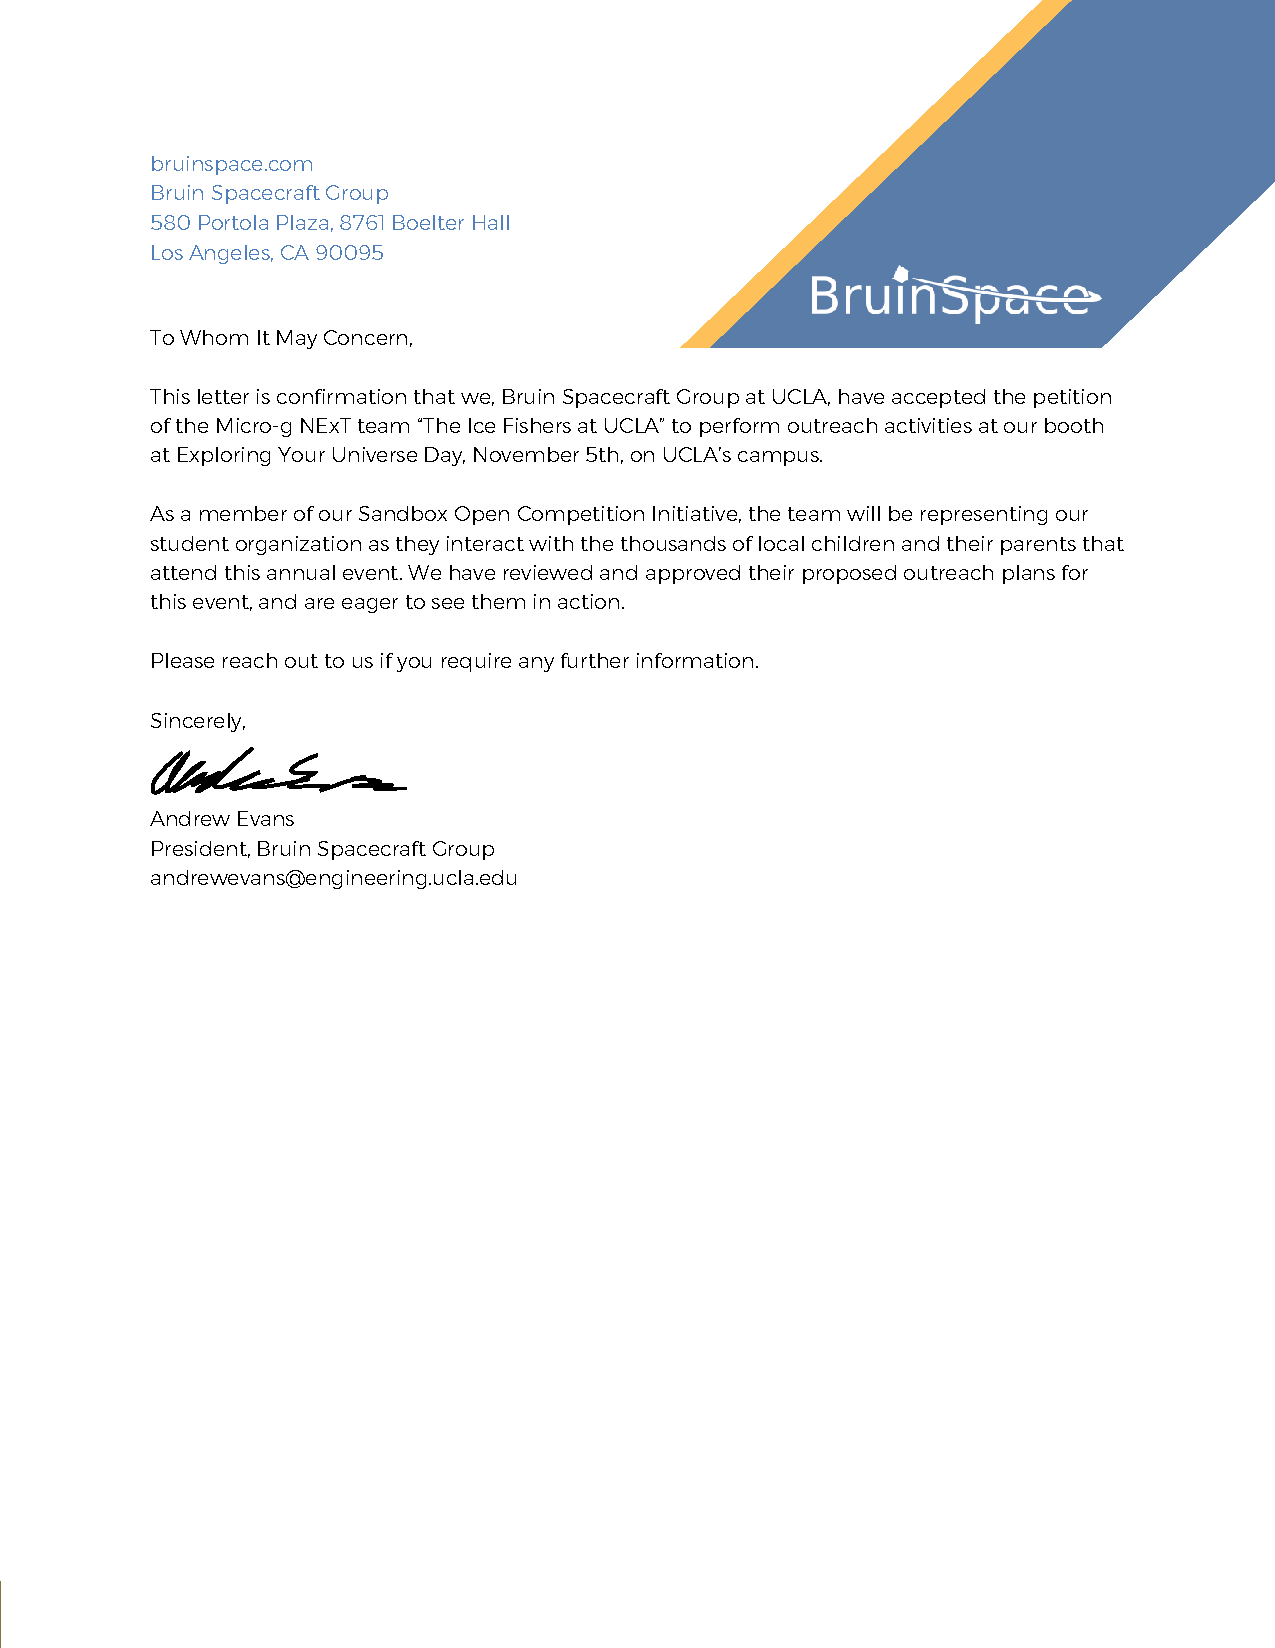
\includepdf{doc1.pdf}
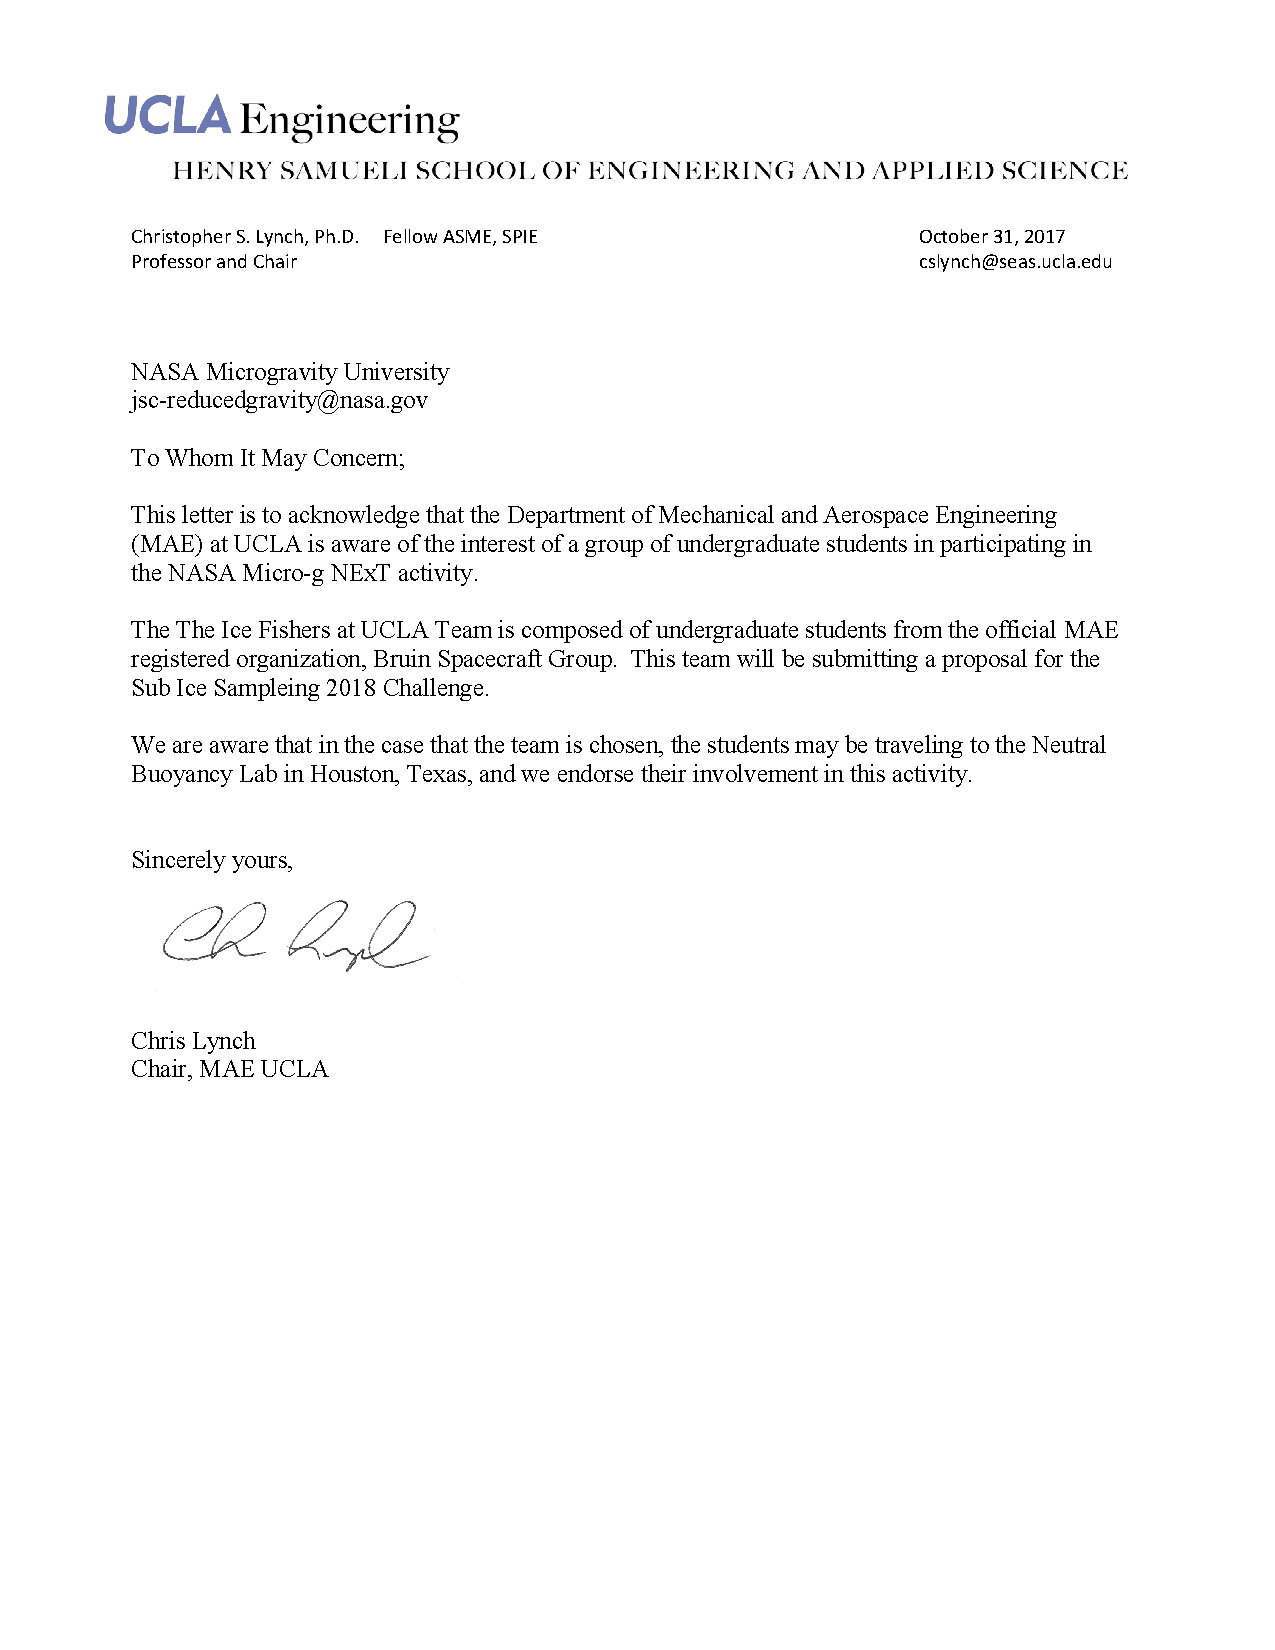
\includepdf{doc2.pdf}
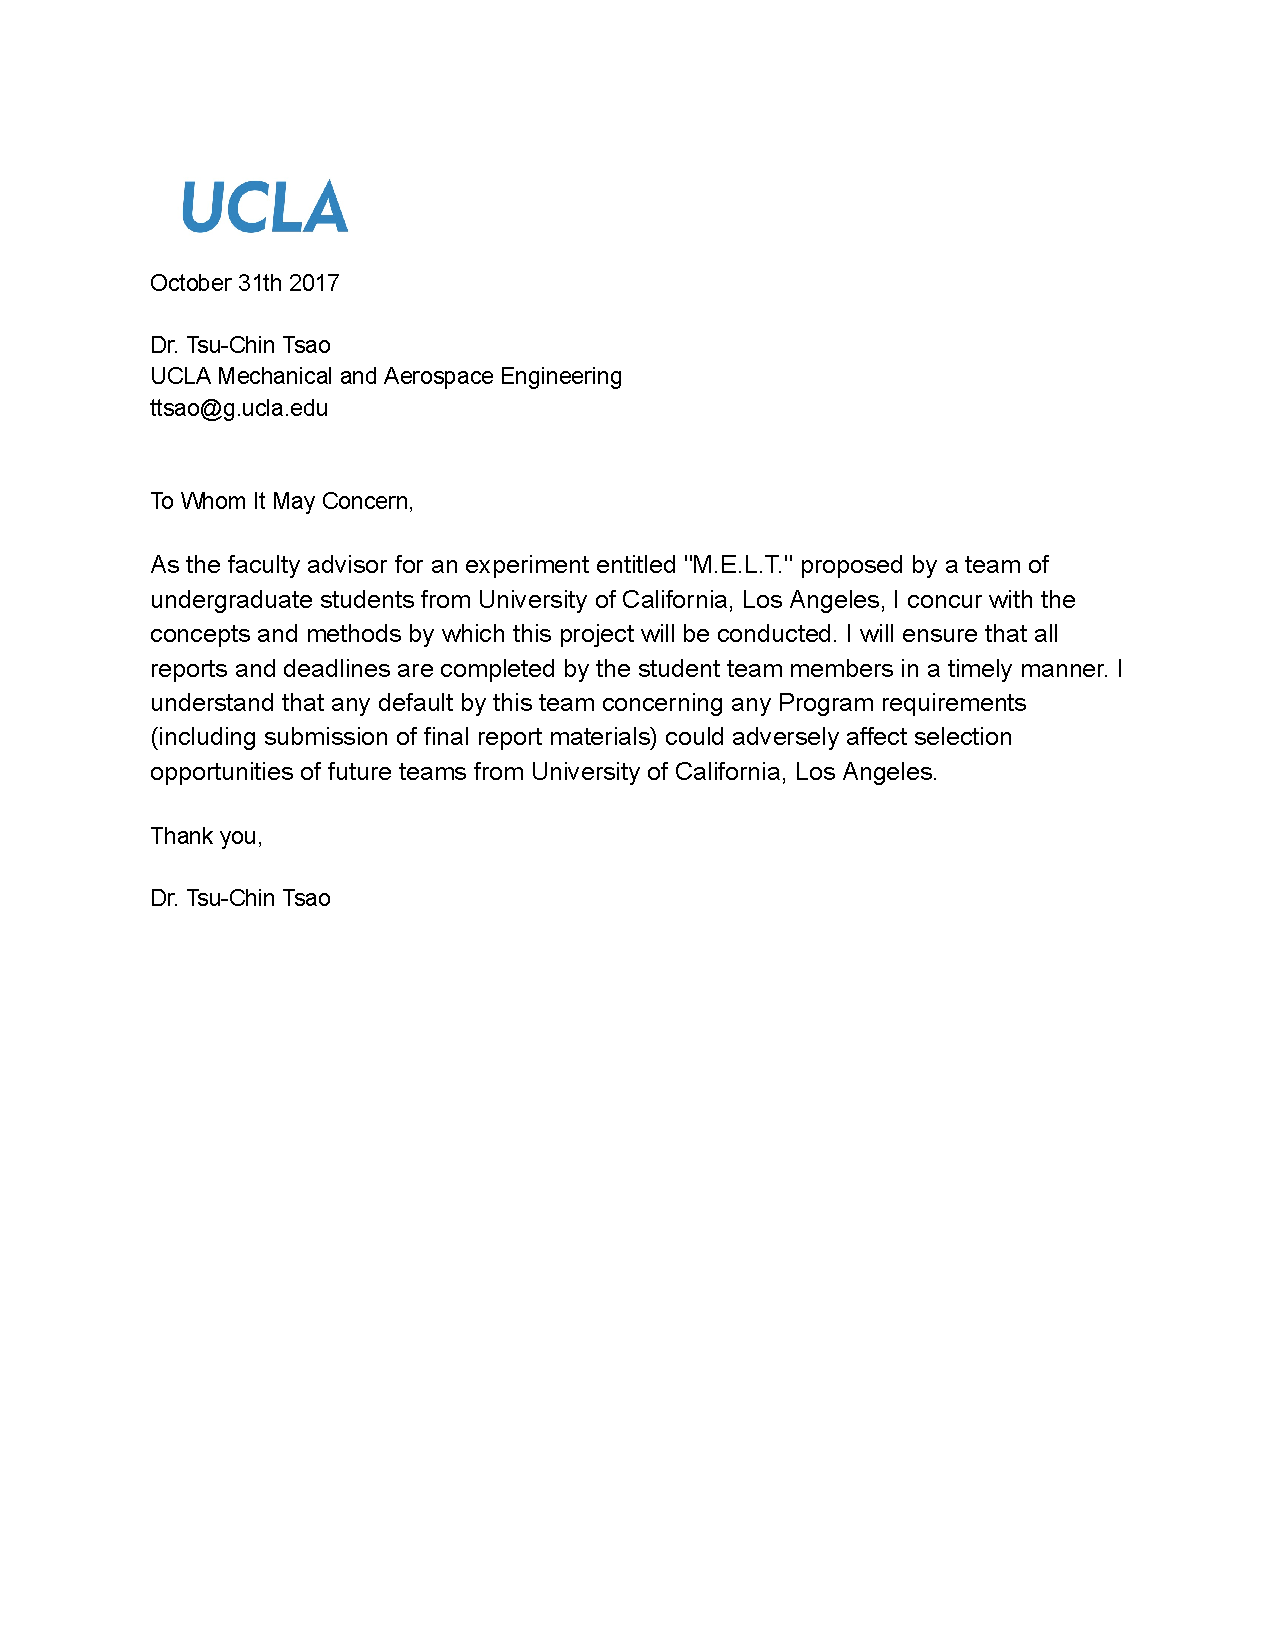
\includepdf{doc3.pdf}

\end{document}
